% ----------------------------------------------------------------
% AMS-LaTeX Paper ************************************************
% **** -----------------------------------------------------------
\documentclass{amsart}
\usepackage{graphicx}
\usepackage{amsmath}
% ----------------------------------------------------------------
\vfuzz2pt % Don't report over-full v-boxes if over-edge is small
\hfuzz2pt % Don't report over-full h-boxes if over-edge is small
% THEOREMS -------------------------------------------------------
\newtheorem{thm}{Theorem}[section]
\newtheorem{cor}[thm]{Corollary}
\newtheorem{lem}[thm]{Lemma}
\newtheorem{prop}[thm]{Proposition}
\theoremstyle{definition}
\newtheorem{defn}[thm]{Definition}
\theoremstyle{remark}
\newtheorem{rem}[thm]{Remark}
\numberwithin{equation}{section}
% MATH -----------------------------------------------------------
\newcommand{\norm}[1]{\left\Vert#1\right\Vert}
\newcommand{\abs}[1]{\left\vert#1\right\vert}
\newcommand{\set}[1]{\left\{#1\right\}}
\newcommand{\Real}{\mathbb R}
\newcommand{\eps}{\varepsilon}
\newcommand{\To}{\longrightarrow}
\newcommand{\BX}{\mathbf{B}(X)}
\newcommand{\A}{\mathcal{A}}
% ----------------------------------------------------------------
\begin{document}

\title{Complex Networks  - Spring 2025\\{\bf Homework 2}}%
\author{Instructor: Jia Liu \\ Solution by: Renan Monteiro Barbosa}%
\date{02/23/2025}

%\dedicatory{}%
%\commby{}%
% ----------------------------------------------------------------

\maketitle
% ----------------------------------------------------------------
\begin{itemize}
\item DUE on 02/23/2025 11:59pm C.T.
\item You can write on the separate work sheet or type your quiz. ( Word or Latex or similar)
\item If you use the handwriting, Solutions must be neat,clear and legible.
\item If you need to scan you quiz, save it as a PDF file. Do not use jpeg, png, jpg etc. Do not submit more than one file.
\item Please check your scanned file before submission. Make sure it is readable, correct order, properly oriented. Make sure it does include all pages.
\item Please name your file as follows: $LastnameInitials-MAP5990quiz1.pdf$.If your name is Alan David Roberts, file name is $RobertsAD-MAP5990quiz1.pdf$.
\item Try to keep the file size less than 4MB.
\item You can resubmit the quiz if you want. Please specify which one is the one to be graded. Otherwise I will grade the most recent version.
\item DO NOT EMAIL me the quiz. All quizzes are submitted via Canvas.
\end{itemize}


\clearpage
\begin{enumerate}

%---------------------------------------------------------------------------------

% ##############################################################################
% Problem 1
% ##############################################################################
\item Demonstrate the following for undirected networks:
\begin{enumerate}
% #######################
% Problem 1-a
% #######################    
\item A 3 regular graph must have an even number of nodes.\vspace{5cm}



% #######################
% Problem 1-b
% #######################
\item The average degree of a tree is strictly less than 2.



\end{enumerate}

\vspace{5cm}

% ##############################################################################
% Problem 2
% ##############################################################################
\item A star graph consists of a single central node with $n-1$ other nodes connected to it. 
\begin{enumerate}
% #######################
% Problem 2-a
% #######################
\item Find the adjacency matrix of the following start network with nodes N:
\begin{figure}[h]
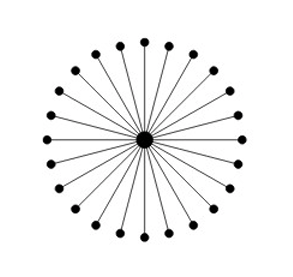
\includegraphics[width=0.3\linewidth]{images/stargraph.PNG}
\end{figure}



% #######################
% Problem 2-b
% #######################
\item Find the largest eigenvalue of the adjacency matrix. 



\end{enumerate}

\clearpage
% ##############################################################################
% Problem 3
% ##############################################################################
\item {\bf Average degree of a growing network} Assume that you are observing a growing undirected network.
The network evolves in time by this simple rules:
\begin{itemize}
\item At time $t = 1$ there is a single isolated node.
\item At each time $t > 1$ a new node is added to the network and is connected
to the existing network by a new link.
\end{itemize}
Consider the network at time $t = T$.
\begin{enumerate}
% #######################
% Problem 3-a
% #######################
\item What is the total number of nodes N? \vspace{0.2cm}

The total number of nodes at Time T will be $N = T$.

\vspace{0.5cm}

% #######################
% Problem 3-b
% #######################
\item What is the total number of links L? \vspace{1cm}

The total number of links L at a particular time T will be $L = T-1$

\vspace{0.5cm}

% #######################
% Problem 3-c
% #######################
\item What is the average degree $\langle k \rangle$? \vspace{0.2cm}

The average degree at a particular time T will be 

$
\langle k \rangle = \frac{2L}{N} = \frac{2\left(T-1\right)}{T}
$

\vspace{0.5cm}

% #######################
% Problem 3-d
% #######################
\item What is the average degree in the limit $T \rightarrow +\infty $? \vspace{0.2cm}

As T approaches infinity the average degree will be:

\vspace{0.2cm}

$
\langle k \rangle = \frac{2L}{N} = \frac{2\left(T-1\right)}{T}
$

\vspace{0.2cm}

$
\lim\limits_{T\to \infty} \langle k \rangle = \lim\limits_{T\to \infty} \frac{2\left(T-1\right)}{T} = 2
$

\vspace{0.5cm}

\end{enumerate}

\vspace{3cm}
% ##############################################################################
% Problem 4
% ##############################################################################
\item One can calculate the diameter of certain types of network exactly. Assume that each of these network has network size N.
\begin{enumerate}
% #######################
% Problem 4-a
% #######################
\item What is the diameter of a fully connected network? \vspace{1cm}

The diameter of a fully connected network is always 1, because every node is directly connected to every other node.

\vspace{0.2cm}

% #######################
% Problem 4-b
% #######################
\item What is the diameter of a star network? \vspace{1cm}

In a star network, the diameter will always be 2. Any node can reach any other node by going through the central hub

% \vspace{0.2cm}

\vspace{0.2cm}

% #######################
% Problem 4-c
% #######################
\item What is the diameter of a linear chain of N nodes? \vspace{0.5cm}

$N-1$

\vspace{0.2cm}

The diameter of a linear chain of N nodes scales linearly with the number of nodes (N). So the furthest two nodes will always be at the ends of the chain, requiring N-1 hops. So the diameter of a linear chain of N nodes is N-1.

\vspace{0.2cm}

% #######################
% Problem 4-d
% #######################
\item What is the small world diameter property? \vspace{0.5cm}

The small world diameter property implies that despite a large number of nodes, the distance between two randomly chosen nodes in a network is unexpectedly short.

\vspace{0.5cm}

We can have an idea by considering a random network which the expected number of nodes up to distance d from our starting node is:

\vspace{0.2cm}

$
N\left(d\right) \approx 1 + k + k^{2} + ... + k^{d} = \frac{k^{d+1} -1}{k -1}
$

\vspace{0.2cm}

Because $ N\left(d\right) $ cannot exeed the total number of nodes in the network the distances cannot be any value. So we can identify the maximum distance (network's diameter) $d_{max}$

\vspace{0.2cm}

$
N\left(d_{max}\right) \approx N
$

\vspace{0.2cm}

As the number k grows very large, $k >> 1$, we can neglect the term (-1) obtaining:

\vspace{0.2cm}

$
k^{d_{max}} \approx N
$

\vspace{0.2cm}

We can then write the diamater of a random network as follows:

\vspace{0.2cm}

$
d_{max} \approx ln \frac{N}{<k>}
$

\vspace{0.2cm}

This is very surprising, because $ ln N << N$ the distances in a random network are orders of magnitude smaller than the size of the network. The diameter depends logarithmically on the system size.


\vspace{1cm}
% #######################
% Problem 4-e
% #######################
\item Which of the above networks are small-world? In another word, which networks have SWDP(Small World Diameter Property)?

\vspace{0.2cm}

From the above network the fully connected network is the only one that has SWDP(Small World Diameter Property).

\vspace{0.2cm}

The star network does not have the WDP(Small World Diameter Property); while it has a small diameter due to its central hub, it lacks the key characteristic of a small-world network, which is a high clustering coefficient.

\vspace{0.2cm}

The linear chain of N nodes does not have the small-world property, because its diameter scales linearly with the number of nodes (N), meaning the average path length between two nodes grows proportionally to N.

\vspace{0.2cm}

\end{enumerate}

\clearpage
% ##############################################################################
% Problem 5
% ##############################################################################
\item Please submit the network for your final project, including the following. This is a group work. Please discuss with your team members but each one needs to submit the individual report. 
\begin{enumerate}
% #######################
% Problem 5-a
% #######################
\item What is your network? \vspace{0.5cm}

Our network represents the airline transportation network in Europe (or Asia), where nodes represent airports and edges represent direct flight routes between them.
This network allows us to analyze how air connectivity is structured in a given region, identify the most critical hubs, and compare its properties to other airline networks.

\vspace{0.5cm}

% #######################
% Problem 5-b
% #######################
\item Where you get the data? \vspace{0.5cm}

We obtained the data from the OpenFlights dataset (https://openflights.org/data.php).

\vspace{0.5cm}

% #######################
% Problem 5-c
% #######################
\item Describe your network including the application area, size, nodes. \vspace{0.5cm}

This flight network is crucial for air traffic analysis, route optimization, transportation planning, and global connectivity studies.
It can be used in pandemic modeling, economic impact studies, and supply chain logistics.

\vspace{0.5cm}

% #######################
% Problem 5-d
% #######################
\item Why you (or your team) want to study this network. \vspace{0.5cm}

By analyzing this network, we can identify bottlenecks, optimize travel efficiency, and gain insights into global air transportation.

\vspace{0.5cm}

\end{enumerate}

\end{enumerate}

\end{document}
% ----------------------------------------------------------------
